\documentclass[a4paper, 12pt]{article}
\usepackage{listings} 
\usepackage{xcolor}
\usepackage{mdframed}
\usepackage{graphicx}
\usepackage{pgfplots}
\usepackage{float}
\usepackage{mathtools}
\usepackage[margin=1.00in]{geometry}
\DeclarePairedDelimiter\ceil{\lceil}{\rceil}
\DeclarePairedDelimiter\floor{\lfloor}{\rfloor}

\definecolor{code-gray}{gray}{0.93}
\begin{document}
\title{ECE 443 - Project \#1}
\author{Collin Heist}
\date{\today}
\maketitle
\pagenumbering{roman}
\tableofcontents
\lstlistoflistings
\newpage
\pagenumbering{arabic}

\section{Design Process}
My general design process was to start with the provided \textbf{rd1\_jim} project, and remove all the \emph{guts}. This left me with the necessary includes, a hardware setup function, and the generic creation of a task and starting of the scheduler. 

I then worked through the listed project requirements. Starting with the hardware requirements, I altered the hardware initialization to establish \textbf{LED1} and \textbf{LED2} as outputs, \textbf{BTN1} and \textbf{BTN2} as inputs. In order to detect the button presses, I also enabled the change notice interrupts on \textbf{BTN1} and \textbf{BTN2}. The code is shown below in Listing~\ref{lst:init-hardware}.

	\begin{mdframed}[backgroundcolor=code-gray, roundcorner=10pt,
								innerleftmargin=5, innertopmargin=5, innerbottommargin=5]	
	\begin{lstlisting}[language=C, caption=Hardware Initialization, tabsize=2, label={lst:init-hardware}]
	static void initHardware() {
		chipKIT_PRO_MX7_Setup();

		PORTSetPinsDigitalOut(IOPORT_G, LED1 | LED2);
		LATGCLR = SM_LEDS;
	
		if (DEBUG_MODE) { 
			PORTSetPinsDigitalOut(IOPORT_B, SM_LEDS);
			LATBCLR = SM_LEDS;
		}
	
		PORTSetPinsDigitalIn(IOPORT_G, BTN1 | BTN2);
	
		mCNOpen(CN_ON,(CN8_ENABLE | CN9_ENABLE), 0);
		mCNSetIntPriority(1);
		mCNSetIntSubPriority(0);
		unsigned int x = PORTReadBits(IOPORT_G, BTN1 | BTN2);
		mCNClearIntFlag();
		mCNIntEnable(1);

		INTEnableSystemMultiVectoredInt();
	}
	\end{lstlisting}
	\end{mdframed}
	
This project's implementation of queues require the queues themselves to be global variables (so many different tasks can access them). In addition to the queues, I also utilize a few variables for detecting button presses using the change notice interrupt. The global variables and change notice ISR is shown below:

\begin{mdframed}[backgroundcolor=code-gray, roundcorner=10pt,
								innerleftmargin=5, innertopmargin=5, innerbottommargin=5]	
	\begin{lstlisting}[language=C, caption=Global Variables and CN ISR, tabsize=2, label={lst:init-hardware}]
	xQueueHandle button1_queue;
	xQueueHandle button2_queue; 

	unsigned int button1_status_prev = 0;
	unsigned int button2_status_prev = 0;

	unsigned int add_to_button1_queue = FALSE;
	unsigned int add_to_button2_queue = FALSE;
	
	void __ISR(_CHANGE_NOTICE_VECTOR, IPL1) CNIntHandler(void) {
		if (DEBUG_MODE) { LATBINV = LEDD; }
	
		hwDelay(DEBOUNCE_TIME_MS);
		unsigned int button1_status_new = PORTG & BTN1;
		unsigned int button2_status_new = PORTG & BTN2;

		if ((button1_status_prev == 0) && (button1_status_new == BTN1))
			add_to_button1_queue = TRUE;
		if ((button2_status_prev == 0) && (button2_status_new == BTN2))
			add_to_button2_queue = TRUE;

		button1_status_prev = button1_status_new;
		button2_status_prev = button2_status_new;

		if (DEBUG_MODE) { LATBINV = LEDD; }
		mCNClearIntFlag();
	}
	\end{lstlisting}
	\end{mdframed}
	
Very simply, a \textbf{DEBOUNCE\_TIME\_MS} millisecond hardware-assisted delay is utilized to account for debounce, and then the current status of buttons is compared with the previous status of both buttons. A change from either button being off (0) to on (\textbf{BTN1} or \textbf{BTN2}) indicates a press occurred, and that button's flag is set to TRUE.
	
The project specifications say that the \textbf{main()} function must create a \emph{single} task and then start the scheduler. The starter task in-turn creates the remaining required tasks. As soon as the task scheduler is started, no more non-tasks are executed, leaving a very empty main that looks like this:

	\begin{mdframed}[backgroundcolor=code-gray, roundcorner=10pt,
								innerleftmargin=5, innertopmargin=5, innerbottommargin=5]	
	\begin{lstlisting}[language=C, caption=Main Function, tabsize=2, label={lst:main}]
	int main() {
		initHardware();

		xTaskCreate(initTask, "Initialization Task",
			configMINIMAL_STACK_SIZE, NULL, 3, NULL);
		vTaskStartScheduler();

		return 0;
	}
	\end{lstlisting}
	\end{mdframed}
	
The initialization task is where I began to run into a few problems. We were given the requirement that the initialization task was to create the required tasks, and then delete itself using \textbf{vTaskDelete()}. However, I constantly received compilation errors (saying the function was not declared) when I used that function. Until I figured out the problem, I simply set the initialization task to a very low priority (1), so that after the other tasks were declared it would just never be entered again. However, this led to the unintended consequence where after I created my first send button task (\textbf{BTN1}), since it was higher priority than my initialization function, the scheduler immediately moved over to that task. This meant no other tasks could be created.

I eventually was able to rectify this problem by setting the initialization task to the highest priority necessary (3), and then adjusting a definition inside the \textbf{FreeRTOS} configuration files that \emph{allowed} for the use of \textbf{vTaskDelete()}. This meant the created tasks were not immediately switched to, and the program was able to continue as expected. My initialization task is shown below, in Listing~\ref{lst:init-task}.

	\begin{mdframed}[backgroundcolor=code-gray, roundcorner=10pt,
								innerleftmargin=5, innertopmargin=5, innerbottommargin=5]	
	\begin{lstlisting}[language=C, caption=Initialization Task, tabsize=2, label={lst:init-task}]
	static void initTask(void *task_params) {
		button1_queue = xQueueCreate(1, sizeof(unsigned int));
		button2_queue = xQueueCreate(1, sizeof(unsigned int));
	
		xTaskCreate(sendButton, "Send BTN1 Task", 
			configMINIMAL_STACK_SIZE, (void *)1, 1, NULL);
		xTaskCreate(sendButton, "Send BTN2 Task", 
			configMINIMAL_STACK_SIZE, (void *)2, 1, NULL);
	
		xTaskCreate(toggleLED, "Toggle LED Task", 
			configMINIMAL_STACK_SIZE, NULL, 2, NULL);
	
		vTaskDelete(NULL);
	}
	\end{lstlisting}
	\end{mdframed}
	
There are a few thing to note in the above code. The queues I created for each button are only capable of holding one item. This is because I implemented my queue receiving function as a higher priority task. This, in combination with a non-zero waiting time for the \textbf{xQueueReceive()} function, mean that as soon as the add-to-queue tasks add to the queue, the LED toggling function will unblock, and parse what is in the queue. Therefore, only a single item will ever be present in each button queue.

Since my \textbf{sendButton()} function is generic (used for both \textbf{BTN1} and \textbf{BTN2}), to create unique behavior I pass in the button number specific to that function, cast as a void pointer, to differentiate the two tasks.

Passing \textbf{NULL} to \textbf{vTaskDelete()} tells \textbf{FreeRTOS} to delete the calling task. This saves the trouble of having to store a pointer to the task as a global variable, and then delete it that way. Once this high priority task is deleted, the \textbf{toggleLED()} function is entered. That is shown below:

\newpage
	\begin{mdframed}[backgroundcolor=code-gray, roundcorner=10pt,
								innerleftmargin=5, innertopmargin=5, innerbottommargin=5]	
	\begin{lstlisting}[language=C, caption=LED Toggle Task, tabsize=2, label={lst:toggleLED}]
	static void toggleLED(void *task_params) {
		unsigned int toggle;
		portBASE_TYPE queue_status;
	
		for(;;) {
			if (DEBUG_MODE) { LATBINV = LEDC; }
				if (button1_queue != 0 | button2_queue != 0) {
					if (xQueueReceive(button1_queue, &toggle,
						(DEBOUNCE_TIME_MS + 1) / portTICK_RATE_MS))
						
				LATGINV = LED1;
					if (xQueueReceive(button2_queue, &toggle,
						(DEBOUNCE_TIME_MS + 1) / portTICK_RATE_MS))
						
				LATGINV = LED2;
			}
		}
	}
	\end{lstlisting}
	\end{mdframed}
	
Following the general layout of a task, this function has two variables that are currently not used but exist for \emph{best-practice}. Because I only place something in either queue if the button should be toggled, the actual value in the queue is superfluous, and so is the status of the queue receive function itself. I chose to wait for a button press in increments of only 21 milliseconds, as this greatly affects the maximum delay between press and toggle. Technically, any value greater than \textbf{DEBOUNCE\_TIME\_MS} (20) milliseconds which is required for debounce just adds unnecessary latency. If either respective queue contains a value, then that respective LED is toggled. Very simple.

Now, my \textbf{sendButton()} function is \emph{slightly} more complicated. This is shown in~\ref{lst:sendButton}.

	\begin{mdframed}[backgroundcolor=code-gray, roundcorner=10pt,
								innerleftmargin=5, innertopmargin=5, innerbottommargin=5]	
	\begin{lstlisting}[language=C, caption=Read Button Task, tabsize=2, label={lst:sendButton}]
	static void sendButton(void *task_params) {
		unsigned int button1_status_new, button2_status_new;
		portBASE_TYPE q_status;
		unsigned int toggle = 1;

		for(;;) {
			if (DEBUG_MODE) {
				if (((unsigned int) task_params) == 1)
					LATBINV = LEDA;
				else
					LATBINV = LEDB;
			}
		
			if ((((unsigned int) task_params) == 1)
				&& add_to_button1_queue) {
				
				q_status = xQueueSendToBack(button1_queue, &toggle, 0);
				add_to_button1_queue = FALSE;
			}
			else if ((((unsigned int) task_params) == 2)
				&& add_to_button2_queue) {
				
				q_status = xQueueSendToBack(button2_queue, &toggle, 0);
				add_to_button2_queue = FALSE;
			}
		
			if (DEBUG_MODE) {
				if (((unsigned int) task_params) == 1)
					LATBINV = LEDA;
				else
					LATBINV = LEDB;
			}
		
			taskYIELD();
		}
	}
	\end{lstlisting}
	\end{mdframed}
	
Once again, the status of adding to the queue is not needed, but included for best-practice. I utilize the \textbf{toggle} variable (which is always 1) as a dummy variable to add to the queue anytime a toggle needs to be initiated. The numerical equivalent of the passed task parameters is then used to check that parameters \emph{add to queue} flag. Then, depending on which button was pressed, the dummy \textbf{toggle} value is added to that respective button's queue, and the flag is reset. But, as previously stated, the actual value placed in the queue is unimportant.

In the event that a value is added to either queue, the \textbf{toggleLED()} task is immediately unblocked, and the queue is emptied. After execution (independent of whether a value was enqueued or not) then the task yields to allow the scheduler to immediately select the \emph{other} button-reading task. This prevents checking only one button repeatedly, until the scheduler moves to the next button. However, on a time-scale this small (1 millisecond task switching) for a HMI, this is likely unnecessary.
 
\section{Testing \& Verification}
In order to verify my program, I used a define statement for \textbf{DEBUG\_MODE} in my main program's header file. In the previously shown Listings, there were various \textbf{if} statements that executed debugging code if that macro was defined.

With this variable defined, various LED's on the board were toggled during the runtime in order to verify the execution of tasks and profile the overall system. I adjusted the LED's as follows:
\begin{enumerate}
\item \textbf{LEDD} - DIO3 - Beginning and end of the change notice interrupt service routine.
\item \textbf{LEDC} - DIO2 - Whenever \textbf{toggleLED()} began its \textbf{for} loop.
\item \textbf{LEDB} - DIO1 - Each loop of \textbf{sendButton()} for \textbf{BTN2}. Both at the start and end of the function's execution.
\item \textbf{LEDA} - DIO0 - Each loop of \textbf{sendButton()} for \textbf{BTN1}. Both at the start and end of the function's execution.
\end{enumerate}

With that in mind, I utilized the \textit{Waveforms} program to capture the following captures. First, the task alternation for each instance of \textbf{sendButton()}. Because of the zero-tick wait time in the \textbf{xQueueSendToBack()} function call, followed by the \textbf{taskYield()}, the two tasks should alternate their execution one after the other. That's what I observed in my testing:
	
\begin{figure}[H]
\centering
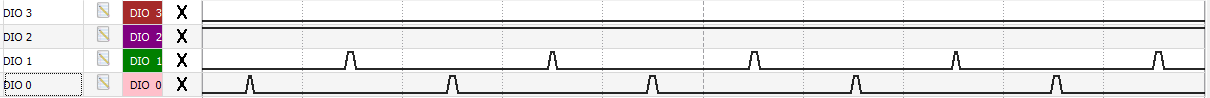
\includegraphics[width=1\textwidth]{img00.png}
\caption{Round-robin task execution of \textbf{sendButtion()} for \textbf{BTN1} and \textbf{BTN2}}
\label{fig:img00}
\end{figure}

The next thing I verified using this method was the frequency at which \textbf{toggleLED()} was called. With no buttons pressed, my code is written such that the queue for button 1 is checked for \textbf{DEBOUNCE\_TIME\_MS}+1 (21) milliseconds, and then button 2 is checked for the same amount of time. My observations support this behavior:

\begin{figure}[H]
\centering
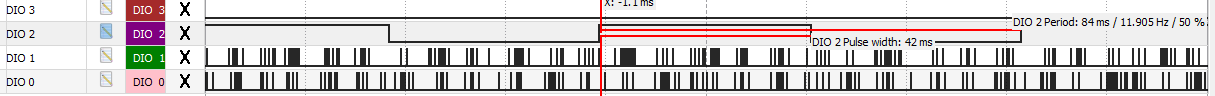
\includegraphics[width=1\textwidth]{img01.png}
\caption{The duration of the \textbf{xQueueReceive()} function calls - 42 milliseconds}
\label{fig:img01}
\end{figure}

Finally, I tested the program's behavior when a button is pressed. For\\ \textbf{DEBOUNCE\_TIME\_MS} milliseconds, no tasks need to be executed. This is because there's no need to check the button add-to-queue flags while the debounce is occurring. This results in the behavior shown in Figure~\ref{fig:img02}.

\begin{figure}[H]
\centering
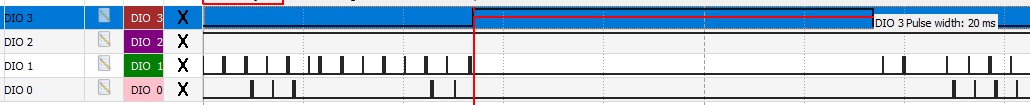
\includegraphics[width=1\textwidth]{img02.png}
\caption{Task execution delay during button debounce.}
\label{fig:img02}
\end{figure}
	
\section{Design Performance}
The designed program performs exactly as specified. Button pressed toggle their respective LED's, and button releases are ignored. In terms of design \emph{limitations}, it is technically possible for the user to press the button and release it (in less than 20 milliseconds) in which no button press would be registered. However, that is nearly impossible for a human to achieve, and it is far more desirable that button debounce be appropriately ignored.

The worst possible latency (in steady-state operation) between a button press and the appropriate LED toggling occurs in a very particular situation. Should the user press the button right after its relevant \textbf{xQueueRecieve()} finished the 21 tick wait. The task's loop would restart, the other button's receive task would need to complete execution (21 ticks, again) and \emph{then} the button press would be acknowledged, toggling the LED.

\end{document}